% !TeX program = xelatex
\documentclass[11pt, a4paper]{article}

% --- Required System Fonts and Geometry ---
\usepackage[a4paper, margin=2.5cm]{geometry}
\usepackage{fontspec}
\usepackage[spanish]{babel}
% --- QFT Mathematics & Formatting Packages ---
\usepackage{amsmath}
\usepackage{amssymb}
\usepackage{physics}   % Automates bra-ket, derivatives, matrices
\usepackage{mathtools}
\usepackage{slashed}   % For Feynman slash notation (e.g., \slashed{p})
\usepackage{graphicx}  % For inserting diagram screenshots later
\usepackage{xcolor}
\usepackage{booktabs}
\usepackage[colorlinks=true, linkcolor=blue, urlcolor=blue, citecolor=blue]{hyperref}

% --- Custom QFT Macros ---
% These will save you hundreds of keystrokes over a semester.
\newcommand{\lag}{\mathcal{L}}          % Lagrangian density
\newcommand{\ham}{\mathcal{H}}          % Hamiltonian density
\newcommand{\hc}{\text{h.c.}}           % Hermitian conjugate
\newcommand{\D}{\mathcal{D}}            % Path integral measure
\newcommand{\del}{\partial}             % Shorthand for partial derivative
\newcommand{\mink}{\eta_{\mu\nu}}       % Minkowski metric

\title{Tería de Campos 1}
\author{Gonzalo Torroba}

\begin{document}

\maketitle
\tableofcontents
\newpage

% ==============================================================================
% INSTRUCTIONS FOR FEDORA:
% When editing locally in TeXstudio, replace the text in each section below 
% with the \input{} command pointing to your transcribed chapter files.
% ==============================================================================

\section{Classical Fields}
% \input{01_classical_fields.tex}

\textit{[Placeholder: On your local machine, create a file named \texttt{01\_classical\_fields.tex}, paste your Gemini/Pix2Tex transcriptions there, and uncomment the \texttt{\textbackslash input} command above.]}

\newpage
\section{Fermion Fields}
% \input{02_fermion_fields.tex}

\textit{[Placeholder: On your local machine, create a file named \texttt{02\_fermion\_fields.tex}, paste your transcriptions there, and uncomment the \texttt{\textbackslash input} command above.]}

\newpage
\section{Campos cuánticos}
\begin{itemize}
    \item Ahora comenzaremos el estudio de teoría cuántica de campos (QFT). El procedimiento es partir de una teoría clásica de campos y ``cuantizarla'' $\rightarrow$ cuantización canónica. Esto da lugar a ``campos cuánticos'', es decir operadores $\hat{\phi}(\vec{x},t)$.
    \item Primero vamos a desarrollar intuición sobre estos campos cuánticos a partir de modelos de materia condensada y sistemas en la red. Luego nos enfocaremos en teorías relativistas.
    \item[*] \textbf{Importante}: en la Naturaleza es al revés; a nivel microscópico la física es cuántica y la descripción clásica emerge como un límite particular $\hbar \rightarrow 0$. Esto va a quedar claro cuando veamos integrales de camino.
    \item[*] Hay sistemas cuánticos que no pueden obtenerse a partir de cuantizar una teoría clásica! (sist. fuertemente interactuantes).
\end{itemize}

\subsection{CAMPOS CUÁNTICOS EN MATERIA CONDENSADA}

\vspace{0.5cm}
\noindent \underline{``Segunda cuantización''}
\begin{itemize}
    \item La representación en término de campos cuánticos es muy útil en sist. cuánticos de muchos cuerpos. Por una confusión histórica, se llama ``segunda cuantización''. Muy mal nombre: nada se cuantiza dos veces.
    \item Consideremos por ejemplo, un sistema de N fermiones idénticos. La función de onda es un determinante de Slater con N! contribuciones:
\end{itemize}
$$ \Psi(x_1 \dots x_N) = \frac{1}{\sqrt{N!}} \begin{vmatrix} \phi_1(x_1) & \dots & \phi_1(x_N) \\ \phi_2(x_1) & \dots & \phi_2(x_N) \\ \vdots & & \vdots \\ \phi_N(x_1) & \dots & \phi_N(x_N) \end{vmatrix} $$
\begin{itemize}
    \item Para una interacción de 2-cuerpos, $V = \sum_{i<j}^N V(r_i - r_j)$, el cálculo de $\matrixel{\Psi}{V}{\Psi}$, $N \sim 10^{23}$, es extremadamente complicado!
    \item Pero en la Naturaleza, en general las interacciones son entre pocos cuerpos, como en V arriba. En ese ejemplo, hay N-2 espectadores, y un cálculo $2 \rightarrow 2$.
    \item[$\Rightarrow$] Este problema se elimina si, en lugar de usar rótulos de partículas utilizamos rótulos usando estados posibles de una partícula.
\end{itemize}

\noindent $\ket{n_1 \dots n_k \dots}$ : $n_k$ partículas en estado $k$ de 1-partícula
\begin{itemize}
    \item Operadores creación y destrucción:

          1) \underline{Bosónicos}: $\ket{n_1 \dots n_k \dots} = (a_1^\dagger)^{n_1} \dots (a_k^\dagger)^{n_k} \dots \ket{0}$
          $$ \comm{a_k}{a_{k'}^\dagger} = \delta_{kk'} \quad , \quad \comm{a_k}{a_{k'}} = 0 $$
          $$ a_k^\dagger \ket{n_1 \dots n_k \dots} = \sqrt{n_k+1} \ket{n_1 \dots n_k+1 \dots} $$
          $$ a_k \ket{n_1 \dots n_k \dots} = \sqrt{n_k} \ket{n_1 \dots n_k-1 \dots} $$

          2) \underline{Fermiónicos}: $\ket{n_1 \dots n_k \dots} = (c_1^\dagger)^{n_1} \dots (c_k^\dagger)^{n_k} \dots \ket{0}$
          $$ \acomm{c_k}{c_{k'}^\dagger} = \delta_{kk'} \quad , \quad \acomm{c_k}{c_{k'}} = 0 $$
          $$ c_k^\dagger \ket{n_1 \dots n_k=1 \dots} = 0 \quad , \quad c_k \ket{n_1 \dots n_k=0 \dots} = 0 $$
          $$ c_k^\dagger \ket{n_1 \dots n_k=0 \dots} = (-1)^{S_k} \ket{n_1 \dots n_k=1 \dots} \quad , \quad S_k = \sum_{i=1}^{k-1} n_i $$

          Las relaciones de (anti) conmutación aseguran la (anti) simetría de la función de onda. Ahora por ejemplo, una interacción $2 \rightarrow 2$ queda
          $$ V = \sum_{k_1 \dots k_4} V_{k_1 \dots k_4} c_{k_1}^\dagger c_{k_2}^\dagger c_{k_3} c_{k_4} $$
          $\rightarrow$ mismos elementos de matriz $\matrixel{\Psi'}{V}{\Psi}$ \\
          $\rightarrow$ elimina automáticamente a los N-2 espectadores \\
          $\rightarrow$ no escalea con N
\end{itemize}

\begin{itemize}
    \item \underline{Sistema con N indefinido} \\
          Hay sistemas donde N no está fijo. Un caso muy importante es el de los fotones del campo electromagnético.
          Al no tener función de onda con N fijo, la única posibilidad es usar la representación anterior con opeardores creación / destrucción.
          $$ H_0 = \int \frac{d^3p}{(2\pi)^3} \omega_p a_p^\dagger a_p \quad , \quad \omega_p = |\vec{p}| $$
          $\rightarrow$ osciladores armónicos, con energía $E_p = \hbar \omega_p$ \\
          Vamos a ver que lo mismo sucede con las demás partículas e interacciones relativistas. \\
          Otros ej. en mat. condensada: ensamble canónico / gran canónico; superconductividad; fonones; $\dots$
    \item Espacio de Fock: para un número indefinido de partículas, el espacio de estados se conoce como \underline{Espacio de Fock},
          $$ \mathcal{F} = \bigoplus_n \mathcal{H}_n \quad , \quad \mathcal{H}_n : \text{espacio Hilbert de n-partículas.} $$
\end{itemize}

\vspace{0.5cm}
\noindent \underline{Cadena armónica y campo escalar}

\noindent Cadena 1D, $N$ átomos masa $m$, espaciado de red $a$.\\
$u_j(t)$ : desplazamiento del átomo $j$ desde equilibrio \\
$p_j(t)$ : momento canónico conjugado.

$$ H = \sum_{j=1}^N \left[ \frac{p_j^2}{2m} + \frac{\kappa}{2} (u_{j+1} - u_j)^2 + \frac{1}{2} m \omega_0^2 u_j^2 \right] $$
donde $\comm{u_j}{p_{j'}} = i\hbar \delta_{jj'} \quad , \quad \comm{u_j}{u_{j'}} = \comm{p_j}{p_{j'}} = 0.$

\begin{itemize}
    \item límite al continuo:
          $$x = ja \quad , \quad a \rightarrow 0$$
          $$\sum_j \to \int \frac{dx}{a},\quad u_j(t) \rightarrow \phi(x,t)$$
          $$ u_{j+1} - u_j = \phi(x+a) - \phi(x) \rightarrow a \pdv{\phi}{x} $$
          $$ \delta_{jj'} \rightarrow a \delta(x-x') \Rightarrow \comm{\phi(x,t)}{p(x',t)} = i\hbar a \delta(x-x') $$
          $\Rightarrow$ Momento canónico del continuo $\pi(x,t) = \frac{p(x,t)}{a}$
          $$ H = \int \frac{dx}{a} \left[ \frac{a^2}{2m} \pi(x,t)^2 + \frac{\kappa a^2}{2} \left( \pdv{\phi}{x}(x,t) \right)^2 + \frac{1}{2} m \omega_0^2 \phi(x,t)^2 \right] $$
          Redefinimos $\frac{a^2} {2m} \pi ^2\to \pi^2$ (término cinético canónico) y para preservar la relación de conmutación, $\left( \frac{a^2}{2m}\right)^{-1}\phi^2\to \phi^2$
          $$ H = \int dx \left[ \frac{1}{2} \pi(x,t)^2 + \frac{1}{2} v^2 (\del_x \phi(x,t))^2 + \frac{1}{2} \tilde{m}^2 \phi(x,t)^2 \right] $$
          $$ \comm{\phi(x,t)}{\pi(x',t)} = i\hbar \delta(x-x') $$
          $$ S = \int dx dt \left\{ \frac{1}{2} (\del_t \phi)^2 - \frac{1}{2} v^2 (\del_x \phi)^2 - \frac{1}{2} \tilde{m}^2 \phi^2 \right\} $$
          \textbf{Campo escalar cuántico no relativista.}

          Además, término anharmónico $u_j^4 \rightarrow$ interacción $\phi^4$
    \item Fonones: cuantos / excitaciones de las vibraciones colectivas de la red.
\end{itemize}

$$ \phi(x) = \int \frac{dk}{2\pi} \frac{1}{\sqrt{2\omega_k}} (a_k e^{ikx} + a_k^\dagger e^{-ikx}) $$
$\comm{a_k}{a_{k'}^\dagger} = {2\pi \delta(k-k')}$ : operadores creación / destrucción de fonones
$$ H = \int \frac{dk}{2\pi} \hbar \omega_k \left( a_k^\dagger a_k + \frac{1}{2} \right) \quad , \quad \omega_k = \sqrt{v^2 k^2 + \tilde{m}^2} $$
Comentario: esta es una versión simplificada de fonones. La teoría completa incluye otros efectos.

\vspace{0.5cm}
\noindent \underline{Líquidos de Fermi}
\begin{itemize}
    \item Consideremos un modelo fermiónico 1D tight-binding:
          $$ H = \underbrace{-t \sum_{j=1}^N (c_j^\dagger c_{j+1} + c_{j+1}^\dagger c_j)}_{\text{hopping}} \underbrace{- \mu \sum_{j=1}^N c_j^\dagger c_j}_{\text{potencial químico}},\quad \acomm{c_j}{c_{j'}^\dagger} = \delta_{jj'} $$

          Se diagonaliza pasando a espacio de momentos:
          $ c_j = \frac{1}{\sqrt{N}} \sum_k e^{ikx_j} \psi_k$, relación de dispersión $E_k = -2t \cos(ka) - \mu$.

          Para una red periódica, $c_{j+N} = c_j \Rightarrow e^{ikNa} = 1 \quad (x_j = ja)$
          $$ \Rightarrow k_n = \frac{2\pi}{a} \frac{n}{N} \quad , \quad k \in \left(-\frac{\pi}{a}, \frac{\pi}{a}\right)\quad , \quad n\in\left(-\frac N 2, \frac N 2 \right) $$
          ya que $k \rightarrow k + \frac{2\pi}{a}$ da el mismo $c_j$.

          \begin{center}
              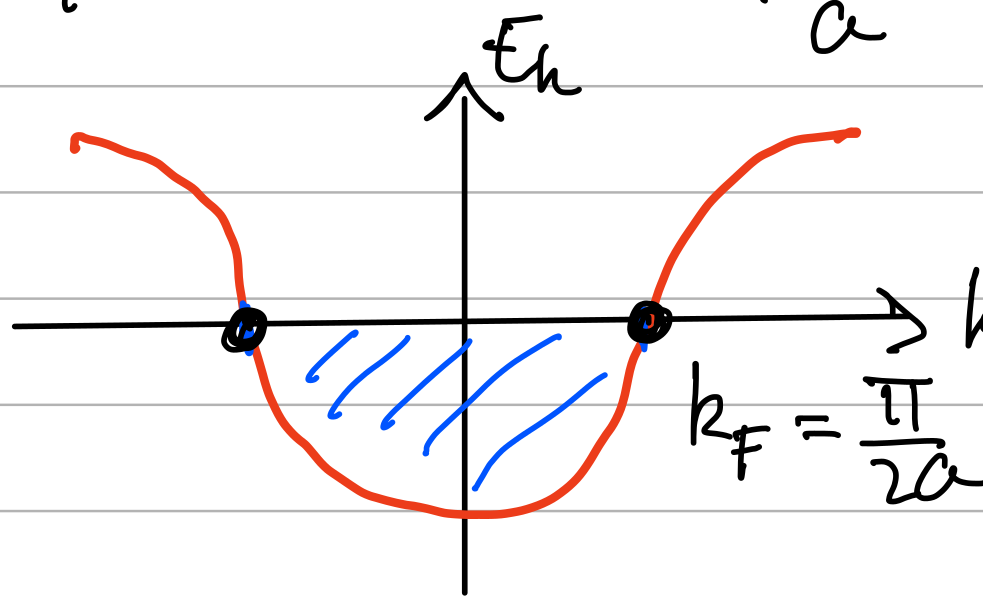
\includegraphics[width=0.6\textwidth]{images/diagram_3_6.png}
          \end{center}

          Si $\mu=0$: medio llenado, $E_{k_F}=0$. Para simplificar nos enfocamos en este caso.
    \item Límite al continuo: $a \rightarrow 0 \Rightarrow E \ll 1/a$ (cutoff)
\end{itemize}

\noindent Sólo los modos con $k \simeq \pm k_F$ se activan ($E \ll 1/a$)
$$ H = \int_{-\pi/a}^{\pi/a} \frac{dk}{2\pi} E_k \psi_k^\dagger \psi_k \simeq \sum_{i=\pm} \int_{-\Lambda}^{\Lambda} \frac{d\tilde{k}}{2\pi} (\pm v_F \tilde{k}) \psi_i^\dagger(\tilde{k}) \psi_i(\tilde{k}) $$
donde $v_F = 2at$ y $k = \tilde{k} \pm k_F$ en la sumatoria, con cutoff $\Lambda \sim 1/a$ \\
Volviendo a espacio posición, $\psi_\pm(x) = \int d\tilde{k} e^{i\tilde{k}x} \psi_\pm(\tilde{k})$
$$ H = -i \sum_{\pm} \int dx \, \psi_\pm^\dagger(x,t) (\pm v_F \del_x) \psi_\pm(x,t) $$
$$ \acomm{\psi_\pm^\dagger(x,t)}{\psi_\pm(x',t)} = \delta(x-x') $$
$$ S = \int dt dx \left[ i \sum_{\pm} \psi_\pm^\dagger(x,t) (\del_t \pm v_F \del_x) \psi_\pm(x,t) \right] $$
\textbf{Campo fermiónico cuántico no relativista.} \\
En este límite $a \rightarrow 0$ podemos re-escalear coordenadas para elegir $v_F = 1$. Se obtiene fermión de Dirac en d=1+1, siendo $\pm$ las dos quiralidades.

\vspace{0.5cm}
\subsection{CAMPO ESCALAR CUÁNTICO RELATIVISTA}
\begin{itemize}
    \item Ahora pasamos a campos cuánticos relativistas en el continuo, es decir operadores $\hat{\phi}(\vec{x},t)$. (En general los escribimos sin $\hat{}$ : $\phi(\vec{x},t)$).
    \item Pero está bueno mantener la intuición de modelos en la red de la sección anterior. Esto corresponde a un cutoff (regularización) en \underline{distancias} $\Delta x \gg a$, \underline{momentos} $p \ll 1/a$. Va a ser útil para ``regularizar'' la teoría, debido a distintos infinitos que aparecen, asociados al número infinito de grados de libertad (en el continuo).
\end{itemize}

\vspace{0.5cm}
\noindent \underline{Cuantización canónica}
\begin{itemize}
    \item Para asegurar la inv. relativista de la teoría cuántica, partimos de la acción invariante de Lorentz (construida a partir de campos), pasamos al Hamiltoniano y cuantizamos. \\
          Consideremos el campo escalar real libre, y luego agregamos interacciones.
          $$ S = \int d^dx \left\{ \frac{1}{2} \eta^{\mu\nu} \del_\mu \phi \del_\nu \phi - \frac{1}{2} m^2 \phi^2 \right\} $$
          $$ \pi(\vec{x},t) = \frac{\delta S}{\delta \dot{\phi}(\vec{x},t)} = \dot{\phi}(\vec{x},t) $$
          $$ H = \int d^{d-1}x \left\{ \pi(\vec{x},t) \dot{\phi}(\vec{x},t) - \lag \right\} $$
          $$ = \int d^{d-1}x \left\{ \frac{1}{2} \pi(\vec{x},t)^2 + \frac{1}{2} (\nabla \phi(\vec{x},t))^2 + \frac{1}{2} m^2 \phi(\vec{x},t)^2 \right\} $$
          Ahora promovemos $\phi, \pi$ a operadores con relaciones de conmutación canónica. Vamos a considerar primero la \underline{representación de Schrödinger}, donde los operadores son independientes de $t$ y los estados evolucionan.
          $$ \hat{H} = \int d^{d-1}x \left\{ \frac{1}{2} \hat{\pi}(\vec{x})^2 + \frac{1}{2} (\nabla \hat{\phi}(\vec{x}))^2 + \frac{1}{2} m^2 \hat{\phi}(\vec{x})^2 \right\} $$
          $$ \Rightarrow \comm{\hat{\phi}(\vec{x})}{\hat{\pi}(\vec{y})} = i \delta^{(d-1)}(\vec{x}-\vec{y}) $$
          $$ \comm{\hat{\phi}(\vec{x})}{\hat{\phi}(\vec{y})} = \comm{\hat{\pi}(\vec{x})}{\hat{\pi}(\vec{y})} = 0 $$
          \noindent $\equiv$ límite al continuo de una red (d-1)-dimensional de osciladores armónicos acoplados, con coeficientes específicos para que sea invariante Lorentz (e.g. $v=c$). \\
          (En general vamos a omitir el $\hat{}$, $\phi$ = operador o función dependiendo del contexto).

\end{itemize}

\begin{itemize}
    \item Operadores creación y destrucción: recordemos que para un \underline{único} oscilador armónico,
          $$ H_1 = \frac{1}{2} p^2 + \frac{1}{2} \omega^2 \phi^2 $$
          el espectro se encuentra escribiendo
          $$ \phi = \frac{1}{\sqrt{2\omega}} (a + a^\dagger) \quad , \quad p = -i \sqrt{\frac{\omega}{2}} (a - a^\dagger) $$
          $$ \comm{\phi}{p} = i \Rightarrow \comm{a}{a^\dagger} = 1 $$
          $$ \Rightarrow H_1= \omega \left( a^\dagger a + \frac{1}{2} \right) \quad , \quad \comm{H_1}{a^\dagger} = \omega a^\dagger \quad , \quad \comm{H_1}{a} = -\omega a $$
          y los autoestados de $H_1$ son $\ket{n} = (a^\dagger)^n \ket{0}$ donde $E_n = (n + \frac{1}{2})\omega$ y el estado fundamental: $\ket{0} : a\ket{0} = 0$

          Para el campo escalar, recordemos la ecuación de movimiento :
          $$ \Box\phi+m^2\phi = 0 \Rightarrow \phi(\vec{x},t) = \int \frac{d^{d-1}p}{(2\pi)^{d-1}} e^{i\vec{p}\cdot\vec{x}} \phi_{\vec{p}}(t) $$
          donde $\phi_{\vec{p}}^* = \phi_{-\vec{p}}$ para que $\phi(\vec{x})^* = \phi(\vec{x})$

          La ecuación de KG queda $\left(\pdv[2]{}{t} + \omega_p^2\right) \phi_{\vec{p}}(t) = 0 \quad , \quad \omega_p = \sqrt{\vec{p}^2 + m^2}$ \\
          $\rightarrow$ Ecuación de  movimiento del oscilador armónico con frecuencia $\omega_p$. Entonces para cada $\vec{p}$ tenemos un oscilador armónico independiente y sabemos cómo cuantizarlo.
\end{itemize}

\noindent Hacemos lo mismo para $\phi(\vec{x})$, donde c/ modo de Fourier se trata como un oscilador indep. con su $a_{\vec{p}}, a_{\vec{p}}^\dagger$ :
$$ \phi(\vec{x}) = \int \frac{d^{d-1}p}{(2\pi)^{d-1}} \frac{1}{\sqrt{2\omega_p}} (a_{\vec{p}} e^{i\vec{p}\cdot\vec{x}} + a_{\vec{p}}^\dagger e^{-i\vec{p}\cdot\vec{x}}) $$
$$ \pi(\vec{x}) = \int \frac{d^{d-1}p}{(2\pi)^{d-1}} (-i) \sqrt{\frac{\omega_p}{2}} (a_{\vec{p}} e^{i\vec{p}\cdot\vec{x}} - a_{\vec{p}}^\dagger e^{-i\vec{p}\cdot\vec{x}}) $$
Notar: $\int_{\vec{p}} (a_{\vec{p}} e^{i\vec{p}\cdot\vec{x}} + a_{\vec{p}}^\dagger e^{-i\vec{p}\cdot\vec{x}}) = \int_{\vec{p}} (a_{\vec{p}} + a_{-\vec{p}}^\dagger) e^{i\vec{p}\cdot\vec{x}}$
$$ \comm{\phi(\vec{x})}{\pi(\vec{y})} = i \delta^{(d-1)}(\vec{x}-\vec{y}) \Leftrightarrow \comm{a_{\vec{p}}}{a_{\vec{p}'}^\dagger} = (2\pi)^{d-1} \delta^{(d-1)}(\vec{p}-\vec{p}') $$
(Probar) Usar: $\int \frac{d^D p}{(2\pi)^D} e^{i\vec{p}\cdot(\vec{x}-\vec{y})} = \delta^D(\vec{x}-\vec{y})$

Reemplazando esta expansión en el Hamiltoniano,
$$ H = \int \frac{d^{d-1}p}{(2\pi)^{d-1}} \omega_p \left( a_{\vec{p}}^\dagger a_{\vec{p}} + \frac{1}{2} \comm{a_{\vec{p}}}{a_{\vec{p}}^\dagger} \right) $$
\begin{itemize}
    \item El segundo término es formalmente divergente; $\comm{a_{\vec{p}}}{a_{\vec{p}}^\dagger} \propto \delta^{(d-1)}(0)$. Viene de sumar energías de punto 0 ($\frac{1}{2}\hbar\omega$) para un número infinito de osciladores (uno en cada sitio).\\
          Además $\int d^{d-1}p \, \omega_p$ también diverge, debido a que $\omega_p \sim |\vec{p}|$ (divergencia ultravioleta).
    \item[*] Este tipo de divergencias UV aparecen mucho en QFT. Una forma de regularizarlas es con la red.
    \item En observables físicos de QFT se cancelan (por ejemplo, diferencias de energías). Pero en presencia de gravedad son importantes. \underline{Problema de la constante Cosmológica}: la teoría cuántica predice $\varepsilon_0$ gigante (controlada por cutoff UV). Pero experimentalmente $\varepsilon_0 \sim 10^{-120} \times \varepsilon_{\text{Planck}}$.
    \item Ej: analizar divergencias IR / UV.
\end{itemize}

\vspace{0.5cm}
\noindent \underline{Espectro de la teoría}
\begin{itemize}
    \item Ya que $\comm{H}{a_{\vec{p}}^\dagger} = \omega_p a_{\vec{p}}^\dagger$, $\comm{H}{a_{\vec{p}}} = -\omega_p a_{\vec{p}}$ el espectro se obtiene como en el caso del oscilador armónico:
    \item[—] Vacío / estado fundamental $\ket{0} :\forall \vec{p}\quad a_{\vec{p}}\ket{0} = 0$. En general se sustrae la energía de punto 0 y entonces $E_0 = 0$.
    \item[—] Estados excitados: $a_{\vec{p}}^\dagger a_{\vec{q}}^\dagger \dots \ket{0}$ tienen $E = \omega_{\vec{p}} + \omega_{\vec{q}} + \dots$. Siempre tienen $E > 0$.\\
        Para enfatizar que $\omega_p$ (frecuencia) define la energía de una excitación, en general vamos a notar $E_{\vec{p}} \equiv \omega_{\vec{p}}$ para estados de 1-partícula.
    \item Operador momento:
          $$ P^i = \int d^{d-1}x \, T^{0i} = -\int d^{d-1}x \, \pi(\vec{x}) \del_i \phi(\vec{x}) $$
\end{itemize}

$$ P^i = \int d^{d-1}x \, p_i a_{\vec{p}}^\dagger a_{\vec{p}} $$
$a_{\vec{p}}^\dagger$ crea estado de momento $\vec{p}$ y energía $\omega_{\vec{p}} = \sqrt{\vec{p}^2 + m^2}\ \equiv$ relación de dispersión relativista para partícula de masa $m$ y momento $\vec{p}$.

\begin{itemize}
    \item \underline{Partículas}: interpretamos a $a_{\vec{p}}^\dagger \ket{0}$ como un estado de una partícula relativista de masa $m$ y momento $\vec{p}$.
    \item Espacio de Hilbert: $\ket{0}, a_{\vec{p}}^\dagger \ket{0}, a_{\vec{p}}^\dagger a_{\vec{q}}^\dagger \ket{0} \dots$ $\rightarrow$ estados multipartícula.
    \item[—] Los $a^\dagger$ conmutan
    \item[—] Un modo $\vec p$ puede contener infinitas partículas.

        $\Rightarrow$ bosones
\end{itemize}

{\centering
\fbox{Partículas $\equiv$ excitaciones de campos cuánticos.}
\par}

\vspace{0.5cm}
\noindent Notar: estas partículas tienen momento $\vec{p}$ definido y no están localizadas en posición (son ondas planas). Se puede formar un paquete de ondas parcialmente localizado:
$$ \ket{\varphi} = \int \frac{d^{d-1}p}{(2\pi)^{d-1}} \varphi(\vec{p}) a_{\vec{p}}^\dagger \ket{0} $$

\vspace{0.5cm}
\noindent \underline{Normalización relativista}:
\begin{itemize}
    \item[—] Elegimos $\braket{0}{0} = 1$.
    \item[—] El estado $a_{\vec{p}}^\dagger \ket{0}$ satisface: $\matrixel{0}{a_{\vec{p}} a_{\vec{q}}^\dagger}{0} = (2\pi)^{d-1} \delta^{(d-1)}(\vec{p} - \vec{q})$
\end{itemize}

\noindent Este producto interno no es invariante de Lorentz.
\begin{itemize}
    \item Queremos que la norma de los estados de partícula sea invariante de Lorentz: \\
          si $p^{\prime \mu} = \Lambda^\mu_{\ \ \nu} p^\nu$ entonces $\ket{p'} = \ket{\Lambda p} = U(\Lambda) \ket{p}$ \\
          con $U$ unitario. Es decir, queremos que las simetrías actúen como operadores unitarios sobre $\mathcal{H}$.
\end{itemize}
Para encontrar la normalización, notamos:
$$ \int d^d p \, \delta(p^2 - m^2) \equiv \text{invariante de Lorentz} . $$
Ahora $p^2 - m^2 = 0$ tiene 2 soluciones: $p_0 = \pm \omega_{\vec{p}}$ \\
Elegimos la rama $p_0 > 0$ (la elección de rama es invariante de Lorentz).
$$ \Rightarrow \int_{p^0 > 0} d^d p \, \delta(p^2 - m^2) = \int \frac{d^{d-1}p}{2p^0} \Bigg|_{p^0 = \omega_{\vec{p}}} \text{ invariante de Lorentz} $$
y entonces $2\omega_{\vec{p}} \delta^{(d-1)}(\vec{p})$ invariante de Lorentz, ya que $$\int \frac{d^{d-1}p}{2\omega_{\vec{p}}} 2\omega_{\vec{p}} \delta^{(d-1)}(\vec{p}) = 1$$.

\noindent $\therefore$ Estados con normalización relativista: $\ket{\vec{p}} = \sqrt{2\omega_{\vec{p}}} a_{\vec{p}}^\dagger \ket{0}$ (El factor $\sqrt{2}$ es por conveniencia).
En particular, la relación de completitud para estados de 1 partícula queda
$$ (\mathbb{I})_{\text{1-part}} = \int \frac{d^{d-1}p}{(2\pi)^{d-1} 2\omega_{\vec{p}}} \ket{\vec{p}}\bra{\vec{p}} $$

\begin{itemize}
    \item Además,
          $$ \phi(\vec{x})\ket{0} = \int \frac{d^{d-1}p}{(2\pi)^{d-1}} \frac{1}{2\omega_{\vec{p}}} e^{-i \vec{p} \cdot \vec{x}} \ket{\vec{p}} $$
          $\Rightarrow$ superposición lineal de estados 1-partícula de momento definido. \\
          Ya que
          $$ \matrixel{\vec{p}}{\phi(\vec{x})}{0} = e^{-i \vec{p} \cdot \vec{x}} $$
          (en analogía con Mecánica Cuántica no relativista, donde $\braket{\vec{p}}{\vec{x}} = e^{-i \vec{p} \cdot \vec{x}}$) \\
          interpretamos:
\end{itemize}
{\centering
\fbox{ $\phi(\vec{x})\ket{0}$ crea una partícula relativista en $\vec{x}$.}
\par}

\vspace{0.5cm}
\subsection{PROPAGACIÓN EN EL ESPACIO-TIEMPO}
\begin{itemize}
    \item Ahora vamos a estudiar la dinámica de campos cuánticos en el espacio-tiempo. Esto se hace pasando a la representación de Heisenberg.
    \item Nos va a permitir entender varios puntos importantes: propagadores, causalidad, ...
\end{itemize}

\noindent \underline{Representación de Heisenberg}
\begin{itemize}
    \item En la representación de Schrödinger tenemos estados que evolucionan y operadores independientes de $t$:
          $$ i \frac{d\ket{\psi}}{dt} = H \ket{\psi} \Rightarrow \ket{\psi(t)} = e^{-iHt} \ket{\psi(0)} . $$
          Representación de Heisenberg: $\matrixel{\psi(0)}{O_H(t)}{\psi(0)} = \matrixel{\psi(t)}{O_S}{\psi(t)}$
\end{itemize}
$$\implies O_H(t) = e^{iHt} O_S e^{-iHt} \quad , \quad i \frac{dO_H}{dt} = \comm{O_H}{H} $$

\newpage
\begin{flushright}
    15.
\end{flushright}

\begin{itemize}
    \item Para el campo escalar,
          $$ \phi(x) \equiv \phi(\vec{x},t) \equiv e^{iHt} \phi(\vec{x}) e^{-iHt} $$
          Los operadores en las dos representaciones coinciden a $t=0$. \\
          y las relaciones de conmutación quedan
          $$ \comm{\phi(\vec{x},t)}{\pi(\vec{y},t)} = i \delta^{(d-1)}(\vec{x}-\vec{y}) $$
          $$ \comm{\phi(\vec{x},t)}{\phi(\vec{y},t)} = \comm{\pi(\vec{x},t)}{\pi(\vec{y},t)} = 0 \quad \text{tiempos iguales} $$
\end{itemize}

\vspace{0.5cm}
\noindent \underline{Evolución del campo escalar libre}
\begin{itemize}
    \item Determinamos la ecuación de movimiento del campo cuántico:
          $$ H = \frac{1}{2} \int d^{d-1}y \left\{ \pi(\vec{y},t)^2 + (\nabla \phi(\vec{y},t))^2 + m^2 \phi(\vec{y},t)^2 \right\} $$
          $$ i \dot{\phi} = \comm{\phi}{H} \quad , \quad i \dot{\pi} = \comm{\pi}{H} $$
          $$ i \frac{\partial}{\partial t} \phi(\vec{x},t) = \comm{\phi(\vec{x},t)}{\frac{1}{2} \int d^{d-1}y \, \pi(\vec{y},t)^2} \quad \text{(los demás términos conmutan)} $$
          $$ = \int d^{d-1}y \, i \delta^{(d-1)}(\vec{x}-\vec{y}) \pi(\vec{y},t) $$
          $$ = i \pi(\vec{x},t) \quad (1) $$
          $$ i \frac{\partial}{\partial t} \pi(\vec{x},t) = \comm{\pi(\vec{x},t)}{\frac{1}{2} \int d^{d-1}y \left\{ \pi(\vec{y},t)^2 + \phi(\vec{y},t)(-\nabla^2 + m^2)\phi(\vec{y},t) \right\}} $$
          $$ = \int d^{d-1}y \left\{ -i \delta^{(d-1)}(\vec{x}-\vec{y}) (-\nabla^2 + m^2)\phi(\vec{y},t) \right\} $$
          $$ = -i (-\nabla^2 + m^2)\phi(\vec{x},t) \quad (2) $$
          (1)+(2): $\frac{\partial^2 \phi}{\partial t^2} = (\nabla^2 - m^2)\phi \Rightarrow (\Box + m^2)\phi(x) = 0$ \\
          ecuación de Klein-Gordon para el campo cuántico \checkmark
\end{itemize}

\newpage
\begin{flushright}
    16.
\end{flushright}

\noindent Recordemos la energía de un estado de 1-partícula con momento $\vec{p}$
$$ E_{\vec{p}} = \omega_{\vec{p}} = \sqrt{\vec{p}^2 + m^2} $$
$$ \comm{H}{a_{\vec{p}}} = -E_{\vec{p}} a_{\vec{p}} \quad , \quad \comm{H}{a_{\vec{p}}^\dagger} = +E_{\vec{p}} a_{\vec{p}}^\dagger $$
$$ \Rightarrow H a_{\vec{p}} = a_{\vec{p}}(H - E_{\vec{p}}) \quad , \quad H^n a_{\vec{p}} = a_{\vec{p}}(H - E_{\vec{p}})^n $$
y similarmente, $H^n a_{\vec{p}}^\dagger = a_{\vec{p}}^\dagger (H + E_{\vec{p}})^n$ \\
\underline{Probar}:
$$ \Rightarrow e^{iHt} a_{\vec{p}} e^{-iHt} = e^{-iE_{\vec{p}}t} a_{\vec{p}} \quad , \quad e^{iHt} a_{\vec{p}}^\dagger e^{-iHt} = e^{+iE_{\vec{p}}t} a_{\vec{p}}^\dagger $$
y entonces
$$ \phi(\vec{x},t) = \int \frac{d^{d-1}p}{(2\pi)^{d-1} \sqrt{2E_{\vec{p}}}} \left( a_{\vec{p}} e^{-i p \cdot x} + a_{\vec{p}}^\dagger e^{+i p \cdot x} \right) \Bigg|_{p^0=E_{\vec{p}}} $$
$\leftarrow$ frecuencia positiva (destruye partícula) \\
$\leftarrow$ frecuencia negativa (crea partícula) \\
El campo cuántico unifica / resuelve la dualidad onda-partícula:
\begin{itemize}
    \item $\phi(x)$ es un operador que, actuando sobre el espacio de Hilbert crea y destruye partículas (excitaciones del campo).
    \item al mismo tiempo, $\phi(x)$ obedece la ecuación de Klein-Gordon y los dos términos en $\phi$ son soluciones de onda.
    \item la función de onda $\Psi$ es un estado del espacio de Hilbert.
\end{itemize}

\vspace{0.5cm}
\noindent \underline{Causalidad}
\begin{itemize}
    \item Un postulado fundamental en Física es causalidad: la causa precede al efecto en todo sistema de referencia.
\end{itemize}

\newpage
\begin{flushright}
    17.
\end{flushright}

\noindent En sistemas clásicos relativistas esto implica: velocidad máxima de propagación es $c$ (velocidad de la luz).
Si el efecto estuviera afuera del cono de luz futuro de la causa, podemos aplicar un boost a otro sistema de referencia para hacer que suceda antes que la causa.

\noindent ¿Qué implica la causalidad en mecánica cuántica?
\begin{itemize}
    \item \underline{Microcausalidad}: dados dos operadores observables $O_1, O_2$
          $$ \comm{O_1(x)}{O_2(y)} = 0 \quad \forall (x-y)^2 < 0 $$
          Requerimos que todos los operadores conmuten si están separados por una distancia tipo espacio. \\
          En mecánica cuántica una medición perturba el sistema. \\
          ¡Una medición en $x$ no puede afectar a una medición en $y$ si $(x,y)$ no están causalmente conectados! \\
          Si tuviéramos $\comm{O_1}{O_2} \neq 0$ para $(x-y)^2 < 0$ un observador en $x$ puede decidir si medir o no $O_1(x)$. Un observador en $y$, midiendo $O_2(y)$ detecta lo que hizo $O_1$ a partir de lo que mide (ya que $O_2 \ket{\psi} \neq O_2 O_1 \ket{\psi}$). \\
          $\Rightarrow$ comunicación a velocidad $> c$.
\end{itemize}

\newpage
\begin{flushright}
    18.
\end{flushright}

\begin{center}
    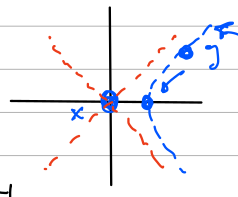
\includegraphics[width=0.6\textwidth]{images/diagram_3_18.png}
\end{center}

\noindent Definimos $\Delta(x,y) \equiv \comm{\phi(x)}{\phi(y)}$ \\
Usando la expresión de $\phi(\vec{x},t)$ en término de $a, a^\dagger$ y la relación de conmutación entre $a, a^\dagger$ \\
(mostrar) $$ \Delta(x,y) = \int \frac{d^{d-1}p}{(2\pi)^{d-1}} \frac{1}{2E_{\vec{p}}} \left( e^{-i p \cdot (x-y)} - e^{i p \cdot (x-y)} \right) $$
\begin{itemize}
    \item $\Delta(x,y)$ invariante de Lorentz sólo puede depender de $s^2 \equiv (x-y)^2$. \\
          Si $s^2 < 0$, hagamos transformación de Lorentz tal que $x^0 = y^0$ \\
          (transformación de Lorentz describe esta hipérbola)
          $$ \Delta(s) = \int \frac{d^{d-1}p}{(2\pi)^{d-1}} \frac{1}{2(\vec{p}^2 + m^2)^{1/2}} \left( e^{i \vec{p} \cdot (\vec{x}-\vec{y})} - e^{-i \vec{p} \cdot (\vec{x}-\vec{y})} \right) $$
          Redefiniendo $\vec{p} \rightarrow -\vec{p}$ en el segundo término, tenemos dos contribuciones iguales y opuestas \\
          $\Rightarrow \Delta(x,y) = 0 \quad \text{si} \quad (x-y)^2 < 0$. \\
          El campo escalar libre respeta causalidad. \\
          (Si $(x-y)^2 > 0 \Rightarrow \Delta(x,y) \neq 0$.)
    \item Causalidad es uno de los axiomas de QFT.
\end{itemize}

\newpage
\begin{flushright}
    19.
\end{flushright}

\noindent \underline{Propagador (función de Wightman)}
\begin{itemize}
    \item Observable importante en QFT: se prepara un estado de 1-partícula en $y$. Amplitud para encontrarla en $x$:
          $$ D(x,y) = \matrixel{0}{\phi(x)\phi(y)}{0} \quad \text{propagador} $$
          Reemplazando las expresiones para $\phi(x), \phi(y)$ con operadores de creación y destrucción, sólo sobrevive
          $$ \matrixel{0}{a_{\vec{p}} a_{\vec{q}}^\dagger}{0} = (2\pi)^{d-1} \delta^{(d-1)}(\vec{p}-\vec{q}) $$
          $$ \Rightarrow D(x,y) = \int \frac{d^{d-1}p}{(2\pi)^{d-1}} \frac{1}{2E_{\vec{p}}} e^{-i p \cdot (x-y)} \quad \text{invariante de Lorentz } \checkmark $$
    \item Comportamiento del propagador: \\
          1) \underline{Adentro del cono de luz}: para $(x-y)^2 > 0$ Como $D(x,y)$ sólo depende de $s^2 = (x-y)^2$, podemos boostear para elegir $\vec{x} = \vec{y} = 0 \quad ; \quad x^0 - y^0 = t > 0$
          $$ \Rightarrow D(x-y) = \int \frac{d^{d-1}p}{(2\pi)^{d-1}} \frac{1}{2(\vec{p}^2 + m^2)^{1/2}} e^{-i (\vec{p}^2 + m^2)^{1/2} t} $$
          La integral sólo depende de $\vec{p}^2 \Rightarrow$ usar coordenadas esféricas:
          $$ \vec{p} = p\hat{n} \quad , \quad \hat{n} \cdot \hat{n} = 1 $$
          $$ D(x-y) = \frac{1}{(2\pi)^{d-1}} \int d^{d-2}\Omega \int_0^\infty dp \, \frac{p^{d-2}}{2(p^2 + m^2)^{1/2}} e^{-i(p^2 + m^2)^{1/2}t} $$
\end{itemize}

\newpage
\begin{flushright}
    20.
\end{flushright}

$$ \int d^{d-2}\Omega = \text{Vol}(S^{d-2}) = \frac{2\pi^{\frac{d-1}{2}}}{\Gamma(\frac{d-1}{2})} $$
$$ \Rightarrow D(x-y) = \frac{\text{Vol}(S^{d-2})}{2(2\pi)^{d-1}} \int_0^\infty dp \, \frac{p^{d-2}}{(p^2 + m^2)^{1/2}} e^{-i(p^2 + m^2)^{1/2}t} $$
Estimación: la integral converge ya que para $p \rightarrow \infty$ se cancelan las oscilaciones rápidas. Para $t \gg m, p \sim m$
$$ D(x-y) \sim m^{d-2} e^{-imt} \quad \text{oscilatorio.} $$

2) \underline{Afuera del cono de luz}: $(x-y)^2 < 0$. Boosteamos a $x^0 - y^0 = 0 \quad , \quad \vec{x} - \vec{y} = r\hat{z}$.
$$ D(x-y) = \frac{1}{2(2\pi)^{d-1}} \int d^{d-2}\Omega \int_0^\infty dp \, \frac{p^{d-2}}{(p^2 + m^2)^{1/2}} e^{i p r \cos\theta} $$
Usar: $d\Omega_{d-2} = d\theta \sin^{d-3}\theta d\Omega_{d-3}$ \\
($d\Omega_{d-2}^2 = d\theta^2 + \sin^2\theta d\Omega_{d-3}^2$)
$$ \Rightarrow D(x-y) = \frac{\text{Vol}(S^{d-3})}{2(2\pi)^{d-1}} \int_0^\infty dp \, \frac{p^{d-2}}{(p^2 + m^2)^{1/2}} \int_0^\pi d\theta \sin^{d-3}\theta e^{i p r \cos\theta} $$
Representación integral: $J_\nu(z) = \frac{(z/2)^\nu}{\sqrt{\pi} \Gamma(\nu + 1/2)} \int_0^\pi d\theta \sin^{2\nu}\theta e^{i z \cos\theta}$
$$ \Rightarrow D(x-y) = \frac{1}{(2\pi)^{\frac{d-1}{2}}} \int_0^\infty dp \, \frac{p^{d-2}}{(p^2 + m^2)^{1/2}} \frac{J_{\frac{d-3}{2}}(pr)}{(pr)^{\frac{d-3}{2}}} $$
Esta integral se puede hacer exacta (da $K_{\frac{d-3}{2}}(mr)$). \\
En el plano complejo, la contribución viene del corte de $(p^2 + m^2)^{1/2}$ en $p = i m$


\newpage
\section{Path Integrals}
% \input{04_path_integrals.tex}

\textit{[Placeholder: On your local machine, create a file named \texttt{04\_path\_integrals.tex}, paste your transcriptions there, and uncomment the \texttt{\textbackslash input} command above.]}

\end{document}